\documentclass[a4paper,titlepage,12pt]{article}
\usepackage[english]{babel}
\usepackage[pdftex]{graphicx}
\usepackage{graphics}
\usepackage[latin1]{inputenc}
\usepackage[T1]{fontenc}
\usepackage{times}
\usepackage{afterpage}
\graphicspath{{./pic/}{../userguide/pic/}{../developerguide/pic/}}
\renewcommand{\topfraction}{0.9}	% 90% of page top can be a float
\renewcommand{\bottomfraction}{0.9}	% 90% of page bottom can be a float
\renewcommand{\textfraction}{0.1}	% only 10% of page must to be text
\title{\textbf{Flat Hunt Redesign \\ and \\ ESDL Extensions}}
\author{Ursina Caluori\\ \href{mailto: ucaluori@student.ethz.ch}{ucaluori@student.ethz.ch}}
\pagestyle{headings}
\usepackage{hyperref}
\hypersetup{
pdfauthor   = {Ursina Caluori <ucaluori@student.ethz.ch>},%
pdftitle    = {Flat Hunt Redesign and ESDL Extensions},%
bookmarks=true,%
bookmarksnumbered=true,%
breaklinks=true,%
colorlinks%
}
%\pdfadjustspacing=1

\begin{document}

  \pdfbookmark[1]{Title Page}{prea}
  \maketitle

  \pdfbookmark[1]{Table of Contents}{toc}
  \tableofcontents
  
  \pagebreak

  \section{Introduction}
    Hello and good day everybody!

  \section{Design Decisions}
    
\paragraph{}
During the redesign of \emph{Flat Hunt} I stumbled upon several tricky issues that had to be dealt with. The more memorable and important ones are described in this chapter.

\subsection{\label{scenes_decision}Singleton Scenes vs. \texttt{last\_scene} vs. no such thing}
\begin{description}
  \item[Singleton scenes:] A class \texttt{SHARED\_SCENES} would provide singleton access to all necessary scenes of the game.
  \item[\texttt{last\_scene}:] Each scene in the game would have an attribute \texttt{last\_scene} with which you could return to the previously run scene. This obviously only works if the scenes' order of appearance has a tree structure.
  \item[No such thing:] You have none of the above. Everytime you change to another scene, a new scene is created.
\end{description}
At the very beginning I was going to use singleton scenes. The main problem with this was, that when you switch to another scene and then come back to a scene already run once, its events are trying to initialize a second time which leads to assertion violations. I tried to overcome this obstacle, but to no avail. Anyway, this problem was also the reason for dropping the \texttt{last\_scene} approach and finally going back to our good old ``create-scenes-like-crazy''-buddy. Whereas the ``like-crazy'' part might be just slightly over the top, since in \emph{Flat Hunt} you really only have three scenes and you switch very rarely. These thoughts are the reason I finally decided to be old-fashioned for once and go with the last approach.

\subsection{Menu Design}
Basically there were three options I took into consideration:

\begin{description}
  \item[1.] Having a class \texttt{MENU} which contains a list of strings (\texttt{EM\_STRING}s to be exact, but could also be generalized to be \texttt{EM\_DRAWABLE}s) that represent the entries. Along with that you would have to store which entry is currently selected. Then you would also need an \texttt{on\_select} - procedure that makes a case distinction based on \texttt{selected\_entry} and reacts accordingly. The code could look like this: 
    \begin{lstlisting}
class
	MENU
...
feature
	entries: ARRAYED_LIST [EM_DRAWABLE]
	
	selected_entry: INTEGER
...
    \end{lstlisting}
    \begin{lstlisting}
class
	MENU_SCENE
...
feature
	menu: MENU
	
	on_select is
		do
			if menu.selected_entry = 1 then
				-- Do what entry 1 says, e.g. start a new game.
	  		elseif menu.selected_entry = 2 then
				-- Do what entry 2 says, e.g. show the credits.
			elseif ...
				...
			end
		end
...
    \end{lstlisting}
  \item[2.] Pretty much the same setup as in case 1, but additionally class \texttt{MENU} would contain a list of agents with each agent corresponding to a menu entry. And \texttt{on\_select} were to be moved from \texttt{MENU\_SCENE} to \texttt{MENU}.
    \begin{lstlisting}
class
	MENU
...
feature
	entries: ARRAYED_LIST [EM_DRAWABLE]
	
	selected_entry: INTEGER
	
	agents: ARRAYED_LIST [PROCEDURE [ANY, TUPLE]]

	on_select is
		do
			agents.i_th (selected_entry).call([])
		end
...
    \end{lstlisting}  
    \begin{lstlisting}
class
	MENU_SCENE
...
feature
	menu: MENU
	
	make is
		do
			create menu.make
			menu.agents.extend (agent agent1)
			menu.agents.extend (agent agent2)
			...
		end
		
	agent1 is
		do
			-- Do what entry 1 says, e.g. start a new game.
		end
		
	agent2 is
		do
			-- Do what entry 2 says, e.g. show the credits.
		end
...	
    \end{lstlisting}

  \item[3.] Case 2 directly leads to a more beautiful solution: Having a class \texttt{MENU} which is an \texttt{EM\_DRAWABLE\_CONTAINER} that contains all menu entries of type \texttt{MENU\_ENTRY}, whereas each menu entry has its callback (i.e. agent) as an attribute. The beauty of this approach is its pure object-orientedness as opposed to the previous two.
    \begin{lstlisting}
class
	MENU_ENTRY
inherit
	EM_DRAWABLE_CONTAINER [EM_DRAWABLE]
...
feature
	callback: PROCEDURE [ANY, TUPLE]
	
	text: EM_STRING
	
	call is
		do
			if callback /= Void then
				callback.call ([])
			end
		end
...	
    \end{lstlisting}    
    \begin{lstlisting}
class
	MENU
inherit
	EM_DRAWABLE_CONTAINER [MENU_ENTRY]
...
feature
	selected_entry: INTEGER
	
	add_entry (a_text: STRING; 
	a_callback: PROCEDURE [ANY, TUPLE]) is
		local
			a_menu_entry: MENU_ENTRY
		do
			create a_menu_entry.make_with_text (a_text)
			a_menu_entry.set_callback (a_callback)
			extend (a_menu_entry)
		end
	
	on_select is
		do
			item (selected_entry).call
		end
...      
    \end{lstlisting}
    \begin{lstlisting}
class
	MENU_SCENE
...
feature
	menu: MENU
	
	make is
		do
			create menu.make
			menu.add_entry (``Entry 1'', agent agent1)
			menu.add_entry (``Entry 2'', agent agent2)
			...
		end

	agent1 is
		do
			-- Do what entry 1 says, e.g. start a new game.
		end
	
	agent2 is
		do
			-- Do what entry 2 says, e.g. show the credits.
		end
...		
    \end{lstlisting}
\end{description}

Originally I implemented the first version, albeit it is the most abominable one, because it seemed to me to be the straight-forward approach (I don't have a very strong object-oriented programming background - or now it is perhaps more appropriate to say I didn't have, because I learned an awful lot by working on this project). It didn't take me very long to notice that this was ugly, so I thought of other solutions and came up with the second and third option. Frankly, I wasn't so sure at this point which one to use, but after discussing the matter with Michela, I finally opted for the third one (which now appears to me should have been the logical choice from the start - but that's just the beauty of hindsight, I guess\ldots).

\subsection{Main Controller Necessary?}
In the old version of \emph{Flat Hunt} a \texttt{MAIN\_CONTROLLER} controlled how the game logic and the visualization worked together. I was not so sure if the main controller was really a necessity, because it seemed to be just as reasonable and also easier to implement if the visualization was directly in contact with the logic behind and got the information on what to display when from there. And also because a \texttt{EM\_SCENE} is not strictly a visualization tool but includes an event loop, which means it is some kind of visualization / control hybrid. So, did I really need some third party controlling unit if my scene can already take care of that?\\
After some contemplation I came to realize that I did indeed need just that, in order to maintain a clear distinction of the \emph{View} and \emph{Controller} clusters (see \autoref{dg_design}), i.e. between visualization and control. 

\subsection{\texttt{PLAYER} and \texttt{PLAYER\_DISPLAYER}}
I had a pretty rough time figuring out how exactly to handle this separation. The main problem was not dividing the model and the view features but more about the question ``Who is in charge?''. I didn't want to have a two-way dependency, because I was told that was bad design. So I could either have a player which has a player displayer as an attribute or the other way around. The logical choice would be to have a player displayer with a player as an attribute (which I also chose in the end), because the player displayer visualizes a player and therefore has to know him. In my first design though, I couldn't eliminate the need for the player to know the displayer. That was until I discovered the \textit{draw} feature of \texttt{EM\_DRAWABLE}s. My original displayer was an \texttt{EM\_DRAWABLE\_CONTAINER [EM\_DRAWABLE]}, and there you don't necessarily have to write your own \textit{draw} procedure (you can, though), you just throw everything that needs to be drawn in the container. The problem with this is that you can't make conditional draws, meaning you have to tell the displayer from the outside when to draw what, so the player needed to inform the displayer about what he wants to get drawn and what not. As I said, my attempts to eliminate the two-way dependency this way failed miserably, so I thought I'd try it the other way around - which obviously was another failure. So then I did a little more research into \emph{EM} and discovered above-mentioned \textit{draw} feature, which worked like a charm and finally allowed me to have my desired one-way dependency.

\subsection{Necessity of \texttt{FLAT\_HUNT\_SCENE}}
A \texttt{FLAT\_HUNT\_SCENE} inherits directly from \texttt{EM\_SCENE}. This class was my prototype for a scene which supports the \texttt{last\_scene} approach described in \autoref{scenes_decision}, but since I decided against that option, this scene was useless for some time. Until, one day, I implemented a simple music player for \emph{Flat Hunt} and wanted it to be a shared music player, so that the songs play on as scenes are switched, and the controls are the same in every scene. That literally called for a \texttt{FLAT\_HUNT\_SCENE}, which is why I dug it out again but changed it profoundly. What is left is a scene that supports a shared music player and its controls. And because that is exactly what I wanted, \texttt{FLAT\_HUNT\_SCENE} is a survivor after all\ldots


  \section{ESDL Extensions}
    Since I first wanted to do my semester thesis on \emph{ESDL}, but then due to several circumstances ended up doing it on \emph{Flat Hunt}, I wanted to keep the option open to simultaneously develop \emph{ESDL} if needed for my project. So I named my thesis ``Flat Hunt Redesign and ESDL Extensions''.\\ 
As I made progress with my work it turned out that \emph{ESDL} already sufficed for \emph{Flat Hunt} in virtually every aspect. And then \emph{ESDL} was transformed into a new project called \emph{EiffelMedia} (\emph{EM}) which would be aggressively developed over summer by a number of people. \\
So basically what I did with \emph{ESDL} was use it, rather than extend it (except for fixing minor bugs which I ran across, but that does not count as an extension in my opinion).\\
In the end, I was relieved that \emph{ESDL}, or now \emph{EM}, already had such good support for everything I needed, because redesigning \emph{Flat Hunt} proved to be much more elaborate than I had imagined.

  \section{Thanks}
    Thanks to\ldots

  \begin{description}
    \item[Michela Pedroni]
      for having been a great assistant who gave me a lot freedom in all aspects and was very supportive.
      
    \item[My Predecessors]
      for their work.

    \item[Till G. Bay]
      for ESDL support and the like.
      
    \item[My Friends, Family and Cats]
      for motivating me and creating a pleasant working atmosphere.
  \end{description}
      
    

  \pdfbookmark[1]{References}{ref}
  \hyperref[ref]{}
  \begin{thebibliography}{150}

  \bibitem{bm03} Bertrand Meyer. \emph{The Outside-In Method of Teaching Introductory Programming}. 2003.\\
    \url{http://www.inf.ethz.ch/~meyer/publications/teaching/teaching-psi.pdf}

  \bibitem{mp03} Michela Pedroni. \emph{Teaching Introductory Programming with the Inverted Curriculum Approach}. ETH Zurich, 2003.\\
    \url{http://se.inf.ethz.ch/projects/michela\_pedroni}
    
  \bibitem{rk05} Roger K�ng. \emph{Touch User Guide}. ETH Zurich, 2005.\\
    \url{http://se.inf.ethz.ch/projects/roger\_kueng}
    
  \bibitem{sa05} Sibylle Aregger. \emph{Redesign of the TRAFFIC library}. ETH Zurich, 2005.\\
    \url{http://se.inf.ethz.ch/projects/sibylle\_aregger}
    
  \bibitem{rb05} Rolf Bruderer. \emph{Object-Oriented Framework for Teaching Introductory Programming}. ETH Zurich, 2005.\\
    \url{http://se.inf.ethz.ch/projects/rolf\_bruderer}
    
  \bibitem{mk04} Marcel Kessler. \emph{Exercise Design for Introductory Programming. "Learn-by-doing" basic OO-concepts using Inverted Curriculum}. ETH Zurich, 2004.\\
    \url{http://se.inf.ethz.ch/projects/marcel\_kessler}

  \bibitem{bb04} Benno Baumgartner. \emph{ESDL - Eiffel Simple Direct Media Library}. ETH Zurich, 2004.\\
    \url{http://se.inf.ethz.ch/projects/benno\_baumgartner}
    
  \bibitem{tgb03} Till G. Bay. \emph{Eiffel SDL Multimedia Library (ESDL)}. ETH Zurich, 2003.\\
    \url{http://se.inf.ethz.ch/projects/till\_bay}

\end{thebibliography}
    

    
  \pagebreak
  
  \appendix
  \section{Flat Hunt User Guide}
      \paragraph{}
  \emph{Flat Hunt} is an application that is used to teach you programming, along with another application named \emph{Touch} \cite{rk05}. \emph{Flat Hunt} is a "Scotland Yard"-like game that will mainly appear in the assignments for the Introduction to Programming course. It is based on \emph{TRAFFIC} \cite{sa05} for modeling the city where the game takes place and on \emph{EiffelMedia} (formerly known as \emph{ESDL} \cite{tgb03}) for visualization.\linebreak[2]

  This document describes how to use \emph{Flat Hunt}.



  \subsection{Introduction}
    Hello and good day everybody!

  \subsection{The Story}
    \emph{As the title suggests (and the introduction mentions), it is all about finding a flat in Zurich\ldots}\\

However, this is not so easy\ldots There is this guy, the estate agent, who is renting flats. The problem is that he is always busy showing flats to other customers, and even in his office they don't really always know where exactly he is. The only thing they know is what kind of transport he is moving around with. This is because the estate agent is taking part in a new VBZ-project called ``Customer tracking''.\\

In collaboration with ETH, they equipped some volunteers with transponders. These transponders gather information like current position and type of transport, and send it in real-time to the office. However, for privacy reasons, only the type of transport can be accessed all the time.\\

Once in a while, the estate agent (\autoref{agent}) calls his office to tell the secretary which flat he is currently visiting. So sometimes, the people there in the office can tell the flat hunters (\autoref{hunters}) where to look for him\ldots

\begin{figure}[h]
\centerline{\hbox{  
  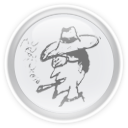
\includegraphics[width=18mm]{agent_white}
  }}
\caption{Estate agent}
\label{agent}
\end{figure}

\begin{figure}[h]
  \centerline{\hbox{
    
\includegraphics[width=135mm]{flat_hunters_white}
  }}
\caption{Flat hunters}
\label{hunters}
\end{figure}

  \subsection{Gameplay}
    \emph{Playing Flat Hunt is not very difficult, especially for those that know the game ``Scotland Yard''\ldots}\\


\subsubsection{General Rules}
 The game lasts for at most 23 rounds. In these 23 rounds, the flat hunters try to find the estate agent, while he tries to avoid them (this is because he would rather rent the flats to elderly couples, since presumably they make fewer parties in the middle of the night\ldots).\\

In each round, every player can make one move on the public transport system. The estate agent is the first, then it's the hunters' turn. One move is either 

\begin{itemize}
  \item  one or two stops by tram (colored lines),
  \item  one stop by train (thick orange lines),
  \item  or one stop by bus (thin light blue lines).
\end{itemize}

A move with a certain transport can only be made if one has still enough tickets (see \autoref{ticket_status}), if there is a connection (obviously), and if there is no other player at that destination (and in the case of tram lines, if there is no hunter in between).\\

 \textcolor{red}{Attention: If you are at a bus-only stop, and you run out of bus tickets, you will get stuck there forever, so be careful\ldots}\\

\begin{figure}[h]
  \centerline{\hbox{
    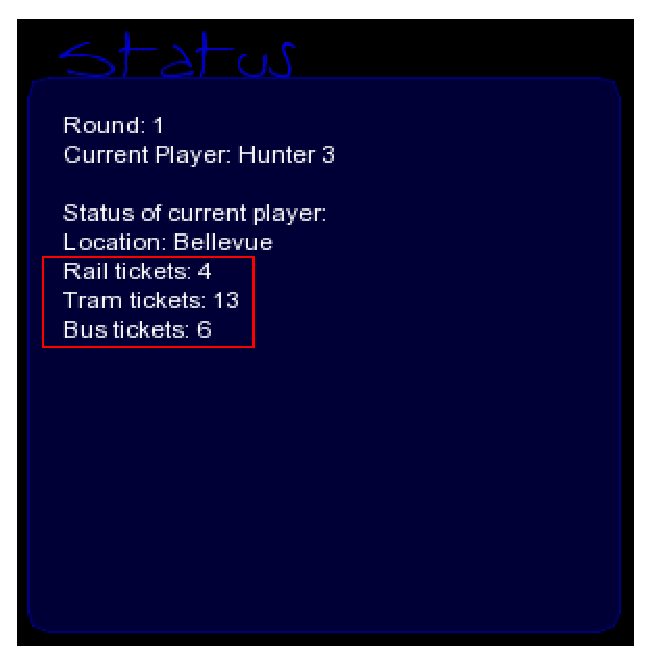
\includegraphics[width=50mm]{ticket_status}
  }}
\caption{Ticket status}
\label{ticket_status}
\end{figure}

The possible places you can move to are colored yellow (see \autoref{highlighted_places}). To make a move, just click on one of those highlighted places. The red circle centers on the player whose turn it is, and in the status box at the right, the game status and information about the current player get displayed. If you want to know the status of another player just click on his picture at the bottom. Click again to close the just opened status box.\\

\begin{figure}[h]
  \centerline{\hbox{
    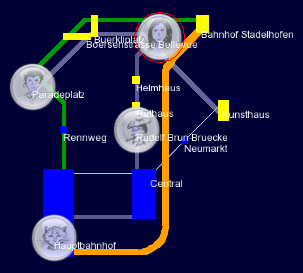
\includegraphics[width=50mm]{highlighted_places}
  }}
\caption{Highlighted places}
\label{highlighted_places}
\end{figure}

The game is over when

  \begin{description}
    \item[a)]the hunters could not find the estate agent within 23 rounds,
    \item[b)]one flat hunter moves onto the place where the agent currently is,
    \item[c)]or the hunters encircle the estate agent so that he cannot move anymore.
  \end{description}

In case a), the winner is the estate agent (he does not have to rent his flat to students), whereas in b) and c) it is the hunters that win, as they get to meet the estate agent on time and thus manage to find a flat.


\subsubsection{\label{game_modes}Game Modes}
There are four modes to play \emph{Flat Hunt}: \emph{Hunt}, \emph{Escape}, \emph{Versus} and \emph{Demo}. Depending on the mode, zero (\emph{Versus}), one (\emph{Hunt/Escape}) or two (\emph{Demo}) parts are taken over by the computer.

  \begin{description}
    
    \item[Hunt]This is probably the most typical situation; the player tries to find the agent, which is played by the computer. Thus, the player only knows about every fifth move where the agent just was\ldots The agent shows himself only in rounds number 1, 3, 8, 13, 18, and 23. In these rounds, the exact route of the agent is displayed under \emph{History} in the status box at the bottom right corner and in the estate agent's own status box if opened. In all other rounds you only see the detailed history up to the round the estate agent last showed himself. As soon as the agent has come out of hiding for the first time, a dimmed version of his picture will always be shown at the location he was last sighted.

    \item[Escape]This is the exact opposite of \emph{Hunt} mode: The agent is played by you, and the hunters are played by the computer. The hunters always move as close in your direction as possible, as they somehow manage to decode your transponder signal, and thus always know your precise location (so much for privacy\ldots). You just have to try to avoid them as long as possible\ldots
  
    \item[Versus]This is the multiplayer mode. One of the players is the agent; the other plays all the hunters. While the player of the agent is making a move, the player of the hunters is supposed to look away\ldots
   
    \item[Demo]This mode is more or less the opposite of the buzzword ``interactive'', but is about as entertaining as watching fish in an aquarium. The computer is playing against himself, trying to catch the agent as fast as possible.
  
  \end{description}

\subsubsection{Other}
  When you run \emph{Flat Hunt}, the first you'll see is a menu (see Figure 7). You can either let the default options in place and just select \emph{start game} or you can adjust the settings to your needs. \emph{Game mode} is explained in \ref{game_modes} Game Modes, \emph{number of hunters} and \emph{map size} should be self-explanatory and \emph{characters} specifies which pictures to use for the players. To toggle between the settings menu and the normal menu press \emph{tab}.\\

  During the game when you press \emph{p}, the pause menu is shown. \emph{Continue} makes the pause menu disappear and lets you resume the game, \emph{new game} takes you to the start menu and \emph{quit} quits the application.\\

  The game over menu is similar to the pause menu, only there is no \emph{continue} in this one.


 
  \subsection{Special Features}
    \subsubsection{Map Control}
Map control is fairly simple: you got two maps in a game scene, one of which only is a smaller version of the other one. The big map is on the left and that's where the action takes place, the little map on the right is meerely a navigation tool. To control the big map, use your mouse as follows:

  \begin{description}
    \item[left click:] only has an impact if clicked on a highlighted place
    \item[richt click + move mouse:] moves map in the direction of your mouse movement
    \item[middle click + move mouse up:] zoom in
    \item[middle click + move mouse down:] zoom out
  \end{description}

  When you \emph{left click + move mouse} in the little map, a light green rectangle is drawn between the point where your left mouse button is pressed down and the point when its released. As soon as you release the mouse button, the map segment that is inside this rectangle gets displayed on the big map.

\subsubsection{Music Player}
\emph{Flat Hunt} comes with an integrated music player and some default background music. Since not everyone likes the same sound, there is also the possibility to play your own.\\ 
Just put your \texttt{.ogg}-files in the directory \texttt{\$\{FLAT\_HUNT\}/resources/sound} before you start the Flat Hunt application. Flat Hunt will then automatically load all the \texttt{.ogg}-files from this directory and play them in alphabetical order (unless you enable shuffle, obviously). Music player control: see \ref{shortcuts} Keyboard Shortcuts.

\subsubsection{\label{shortcuts}Keyboard Shortcuts}
During the game, the following shortcuts are available:

  \begin{description}
    \item[p:] pause the game and show pause menu
    \item[s:] music player toggle shuffle
    \item[v:] music player decrease volume
    \item[shift + v:] music player increase volume (at startup the volume is already at maximum)
    \item[page up:] music player next song
    \item[page down:] music player previous song
    \item[q:] quit the application
  \end{description}


  \subsection{Legal Stuff and Thanks}
    This document is based upon its prior version, which was written by Michela Pedroni and Marcel Kessler (thanks!). All graphics for the game were designed by me and Photoshop. The code of \emph{Flat Hunt} is based on its prior version \cite{mk04}, which is mainly the work of Marcel Kessler. Major parts had to be rewritten by me though.\\

Thanks to Michela Pedroni for her assistance, all my predecessors for their work, Till G. Bay (and others) for the \emph{EiffelMedia} Library (formerly \emph{ESDL} \cite{tgb03}\cite{bb04}) and Bertrand Meyer for the \emph{Eiffel} language. 


 
  \pdfbookmark[2]{References}{ugref}
  \hyperref[ugref]{}
    \begin{thebibliography}{150}

  \bibitem{bm03} Bertrand Meyer. \emph{The Outside-In Method of Teaching Introductory Programming}. 2003.\\
    \url{http://www.inf.ethz.ch/~meyer/publications/teaching/teaching-psi.pdf}

  \bibitem{mp03} Michela Pedroni. \emph{Teaching Introductory Programming with the Inverted Curriculum Approach}. ETH Zurich, 2003.\\
    \url{http://se.inf.ethz.ch/projects/michela\_pedroni}
    
  \bibitem{rk05} Roger K�ng. \emph{Touch User Guide}. ETH Zurich, 2005.\\
    \url{http://se.inf.ethz.ch/projects/roger\_kueng}
    
  \bibitem{sa05} Sibylle Aregger. \emph{Redesign of the TRAFFIC library}. ETH Zurich, 2005.\\
    \url{http://se.inf.ethz.ch/projects/sibylle\_aregger}
    
  \bibitem{rb05} Rolf Bruderer. \emph{Object-Oriented Framework for Teaching Introductory Programming}. ETH Zurich, 2005.\\
    \url{http://se.inf.ethz.ch/projects/rolf\_bruderer}
    
  \bibitem{mk04} Marcel Kessler. \emph{Exercise Design for Introductory Programming. "Learn-by-doing" basic OO-concepts using Inverted Curriculum}. ETH Zurich, 2004.\\
    \url{http://se.inf.ethz.ch/projects/marcel\_kessler}

  \bibitem{bb04} Benno Baumgartner. \emph{ESDL - Eiffel Simple Direct Media Library}. ETH Zurich, 2004.\\
    \url{http://se.inf.ethz.ch/projects/benno\_baumgartner}
    
  \bibitem{tgb03} Till G. Bay. \emph{Eiffel SDL Multimedia Library (ESDL)}. ETH Zurich, 2003.\\
    \url{http://se.inf.ethz.ch/projects/till\_bay}

\end{thebibliography}
    



  
  \pagebreak
  
  \section{Flat Hunt Developer Guide}
    \paragraph{}
\emph{TRAFFIC} \cite{dgsa05}, \emph{Touch} \cite{dgrk05} and \emph{Flat Hunt} is software that hopefully makes learning to program more fun and more interesting for you. \emph{TRAFFIC} is a library that supports the reading and display of public transportation systems. A library is a piece of software whose functionality can be used by other software. \emph{Flat Hunt} is an application that uses the \emph{TRAFFIC} library to model a city map. For the visualization the \emph{EiffelMedia} Library (formerly known as \emph{ESDL} \cite{dgtgb03}\cite{dgbb04}) is used. \emph{Flat Hunt} is a strategy game, similar to Scotland Yard, but with a different background story (for more information about the story and gameplay of \emph{Flat Hunt}, read the Flat Hunt User Guide). \emph{Touch} is also an application that uses the \emph{TRAFFIC} library. For more information on \emph{TRAFFIC} and \emph{Touch}: see \cite{dgsa05} and \cite{dgrk05} or visit this website: \htmladdnormallink{http://se.inf.ethz.ch/traffic}{http://se.inf.ethz.ch/traffic}.\\

  This document describes how \emph{Flat Hunt} is built, what classes are important and highlights some of their features.

\pagebreak

  
  \subsection{Getting Started}
    \emph{What you need for running \emph{Flat Hunt}\ldots}


\subsubsection{Requirements}
\begin{description}
  \item[EiffelStudio:] \url{http://www.eiffel.com/downloads/}
  \item[TRAFFIC:] \url{http://se.inf.ethz.ch/traffic/}
  \item[EiffelMedia:] \url{http://se.inf.ethz.ch/eiffelmedia/}
\end{description}

\subsubsection{Installation}
\emph{EiffelStudio}, as well as \emph{EiffelMedia}, come with an installer. Just follow the onscreen instructions like you would when installing any other program. No magic there..\\

\emph{TRAFFIC} does not need to be installed, just download the zip-file and unzip it to a directory of your choice.\\ 
Flat Hunt is located in the directory \texttt{traffic/example/flat\_hunt}. To get it to run, however, you'll have to compile it first.\\

For that you have to complete the following steps:

\begin {enumerate}
	\item{Start EiffelStudio}
	\item{Click on "File ->New Project...". Choose "Open existing Ace (control file)" from the dialog (see \autoref{newproject}) and click on "Next".
\begin{figure}[h]
\centerline{\hbox{  
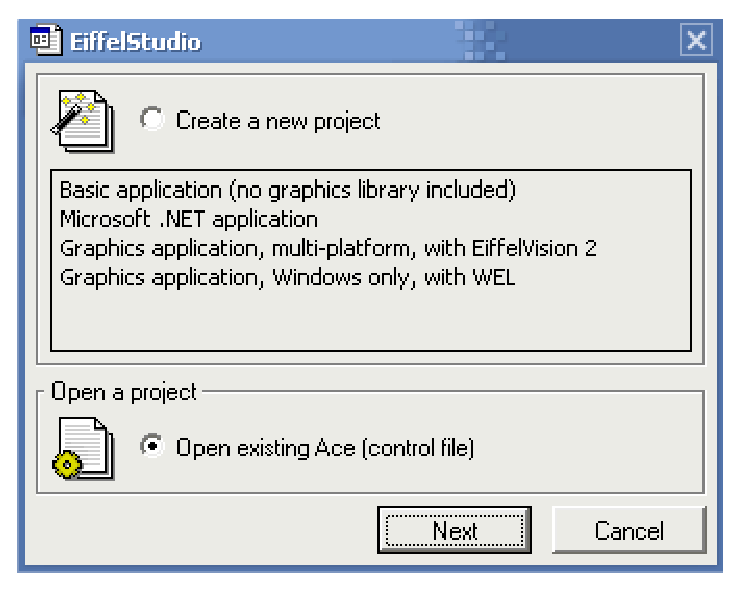
\includegraphics[width=80mm]{new_project}
  }}
\caption{New Project Dialog}
\label{newproject}
\end{figure}	  
}
	\item {This will open a file dialog that lets you choose the Ace file. Browse to the directory \texttt{traffic/example/flat\_hunt}. Depending on the operating system you are working on, choose \emph{ise\_windows.ace} or \emph{ise\_linux.ace}. Click on "Open". }
	\item{The dialog shown in \autoref{choosedir} lets you choose the project directory. In most cases you can leave both paths (Ace file and location) as EiffelStudio proposes. Make sure that the checkbox for compiling the generated project is selected. Click on "OK". This will start the compilation of the project.
\begin{figure}[h]
\centerline{\hbox{  
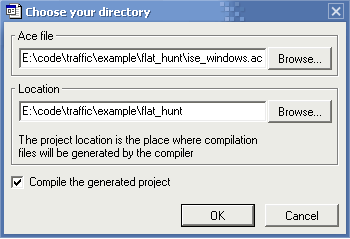
\includegraphics[width=80mm]{choose_directory}
  }}
\caption{Project Directory Dialog}
\label{choosedir}
\end{figure}
}
	\item{Once the project is compiled you can execute it by clicking on the "Launch" button in EiffelStudio or by hitting \textbf{F5}.}
\end {enumerate}

Now you are ready for playing Flat Hunt. Enjoy\ldots 



  \subsection{Design}
    \subsubsection{Overview}
When opening \emph{Flat Hunt} in EiffelStudio, the cluster view in the bottom left corner of EiffelStudio shows many clusters. For you only the top-level clusters \emph{Traffic} and \emph{Flat\_hunt} are important.\\

To remove complexity, \emph{Flat Hunt} is structured in three clusters (see Figure 1): \emph{Model}, \emph{View} and \emph{Controller}. In each cluster, there are several classes, and sometimes there are subclusters.


\subsubsection{Controller cluster}
Cluster \textbf{Controller} is the fundamental cluster in \emph{Flat Hunt}. Here are the classes that ``control'' the actions. They make sure that the displayer classes in cluster \textbf{View} display the proper information, which they get from the \textbf{Model} classes. For example, feature \textit{prepare} in class \texttt{MAIN\_CONTROLLER} controls the display update by calling \textit{game\_scene.center\_on\_player (game.current\_player)}.

\begin{itemize}
  \item{\textbf{MAIN\_CONTROLLER}: The \texttt{MAIN\_CONTROLLER} is (as the name suggests) responsible for many things. It provides access to the \texttt{GAME\_SCENE}, to class \texttt{GAME} and to the whole \emph{TRAFFIC} library, which is responsible for the visualization of the map.}
  \item{\textbf{GAME}: Class \texttt{GAME} features the game logic. It knows which player's turn it is, and also, since it is an heir of \texttt{GAME\_CONSTANTS}, what state the game is in.}
\end{itemize}

\begin{figure}[h]
\centerline{\hbox{  
  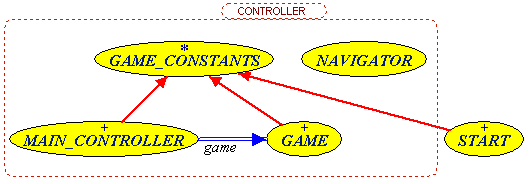
\includegraphics[width=135mm]{controller}
  }}
\caption{Diagram of the Controller Cluster}
\label{controllerdiagram}
\end{figure}

\subsubsection{Model cluster}
In the cluster \textbf{Model}, there are two important parent classes: Class \texttt{PLAYER} and class \texttt{BRAIN}. \texttt{PLAYER} is the parent of \texttt{FLAT\_HUNTER} and \texttt{ESTATE\_AGENT}, and \texttt{BRAIN} is the parent of \texttt{HUMAN}, \texttt{FLAT\_HUNTER\_BOT} and \texttt{ESTATE\_AGENT\_BOT}. These \textbf{Model} classes describe the internal representation of ``real world'' objects. Here is a description of some of these classes.

\begin{itemize}
  \item{\textbf{PLAYER}: Class \texttt{PLAYER} knows the basic things one needs to know about a player of \emph{Flat Hunt}, like how many tickets he got left. It features the commands \textit{play} and \textit{move} and has either a \texttt{HUMAN} or a \texttt{BOT} brain.}
  \item{\textbf{ESTATE\_AGENT}: This is one of the two heirs of class \texttt{PLAYER}. It has some additional information that is special for an estate agent player like knowing where he last showed himself.}
  \item{\textbf{BRAIN}: Class \texttt{BRAIN} includes the intelligence to choose the next move.}
\end{itemize}

\begin{figure}[h]
\centerline{\hbox{  
  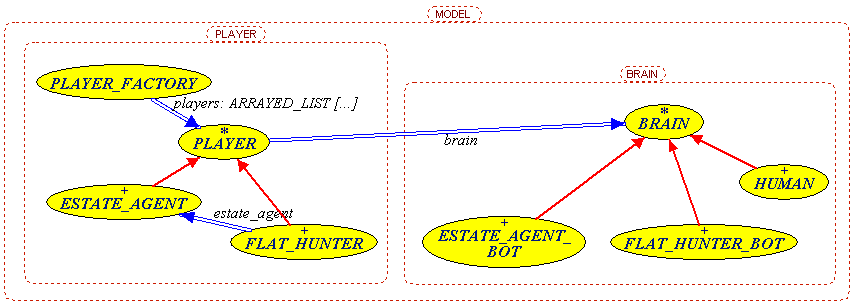
\includegraphics[width=135mm]{model}
  }}
\caption{Diagram of the Model Cluster}
\label{modeldiagram}
\end{figure}

\subsubsection{View cluster}
 This clusters job is to make sure that the user sees what is going on. It includes all scenes and menus, as well as displayers for the game players and status information.

\begin{itemize}
  \item{\textbf{PLAYER\_DISPLAYER}: This class displays the player on the map and prints the amount of tickets left. \texttt{PLAYER\_DISPLAYER} knows this information because of the client-supplier relationship with class \texttt{PLAYER}.}
  \item{\textbf{GAME\_SCENE}: Contains all the drawables of the current game scene and displays them.}
\end{itemize}

\begin{figure}[h]
\centerline{\hbox{  
  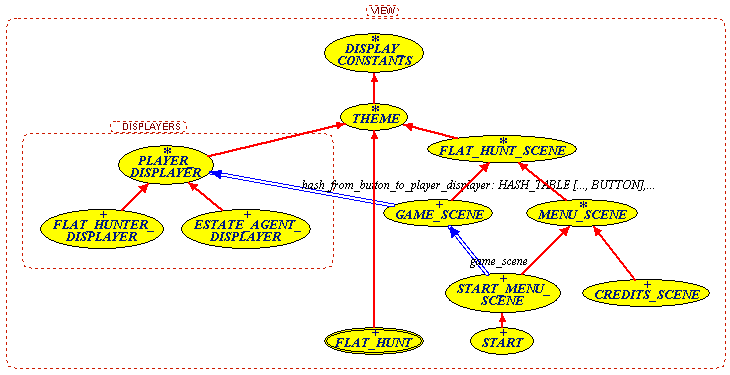
\includegraphics[width=135mm]{view}
  }}
\caption{Diagram of the View Cluster}
\label{viewdiagram}
\end{figure}

\subsubsection{Util}
Those classes that are not directly part of the game, but rather serve as utils, reside in the \textbf{Util} cluster. For one, there are several menu handling classes, which provide the functionality for a normal menu and an option menu. Also important are the helper classes like \texttt{TEXT\_BOX}, which allows to comfortably display status messages in a nice translucent box. And last but not least, a basic music player with shuffle function can be found here.


  \subsection{The States of the Game}
    \subsubsection{Overview}
Every game has at least two states: playing and game over. \emph{Flat Hunt} has six states in total; three playing states and three game over states (see Figure x). These game states are defined in class \texttt{GAME\_CONSTANTS}:

\texttt{Agent\_stuck, Agent\_stuck, Agent\_caught, Agent\_escapes, Prepare\_state, Play\_state, Move\_state: INTEGER is unique}


\subsubsection{Game Loop}
For each player in each round in \emph{Flat Hunt}, the game goes through the following states: \texttt{Prepare, Play} and \texttt{Move}. In addition, there are three game over states: \texttt{Agent\_stuck, Agent\_caught} and \texttt{Agent\_escaped}.

\begin{description}
    
  \item[Prepare] If the game is in this state, the current player gets a red circle and the possible moves are calculated and displayed. If the current player is the estate agent, and there are no possible moves, the agent is stuck and thus the game is over (state \texttt{Agent\_stuck}). If that is not the case, the game goes in state \texttt{Play}.
  
  \item[Play] In this state, if the current player is played by a human, the game waits until the human player clicks on one of the places that are highlighted. If the player is controlled by an artificial intelligence, then the best of the possible moves is calculated. The game then goes in state \texttt{Move}.
  
  \item[Move] In this state, the move selected in state \texttt{Play} is performed. After the move, the game checks if the player hits the place of the estate agent. If that is the case, the game goes into state \texttt{Agent\_caught}. If the agent did not get caught, and the round number is greater than 23, then the estate agent is the winner and the game goes into state \texttt{Agent\_escaped}. If none of the above is the case, then it's the next player's turn and the game loop starts again in state \texttt{Prepare}.

\end{description}

In the classes \texttt{MAIN\_CONTROLLER}, \texttt{GAME} and \texttt{PLAYER}, you can find the features \textit{prepare}, \textit{play} and \textit{move} that deal with these game states. As an example, let's have a look at feature \textit{move} in class \texttt{GAME}:\\

\begin{lstlisting}
move is
		-- Make the chosen move.
	do
		if current_player = estate_agent then
			update_agent_visibility
		end
		current_player.move
		if current_player.location = estate_agent.location 
		and current_player /= estate_agent then
			state := Agent_caught
			update_agent_visibility
		else
			state := Prepare_state			
		next_turn
	end    
end             
\end{lstlisting}

 
  \subsection{Guided ``Walk-Through''}
    \emph{What happens when you start \emph{Flat Hunt}? In this last chapter we will go step-by-step through a typical \emph{Flat Hunt} game. However, because there are lots of details involved, we concentrate on the more important steps\ldots}

\begin{enumerate}
  \item At the very beginning, the application has to be launched. By calling\\ \textit{make\_and\_launch} of the root class \texttt{FLAT\_HUNT} exactly that is achieved. This feature sets the application name, resolution and several other options and then launches the first scene to be displayed, which is of type \texttt{START} and is an heir of \texttt{START\_MENU\_SCENE}.
  \item When ``start game'' is selected in this scene, \textit{start\_callback} is called and creates a game with the proper settings and a game scene, whose job it is to visualize the game. \textit{start\_callback} also creates the \texttt{MAIN\_CONTROLLER} and calls \textit{main\_controller.start\_game}.
  \item \textit{start\_game} in class \texttt{MAIN\_CONTROLLER} calls \textit{create\_players} as well as \textit{start\_game} of class \texttt{GAME}. Those create the players using class\\ \texttt{PLAYER\_FACTORY} and set the game state to \texttt{Prepare\_state}.
  \item In class \texttt{PLAYER\_FACTORY}, for example the estate agent is created using \textit{estate\_agent.make} in feature \textit{build\_players}.
  \item This creates a \texttt{HUMAN}, \texttt{FLAT\_HUNTER\_BOT} or \texttt{ESTATE\_AGENT\_BOT} brain depending on the value of \texttt{flat\_hunters\_bot} or\\ \texttt{estate\_agent\_bot} respectively, which are boolean values to indicate if a human or the computer is going to play the corresponding player(s).
  \item Back to class \texttt{MAIN\_CONTROLLER}: Feature \textit{idle\_action} gets called whenever nothing is going on, i.e. now. \textit{idle\_action} checks whether the game is in one of the three game loop states, and calls the corresponding feature in class \texttt{MAIN\_CONTROLLER}. In the first run, this is \textit{prepare}\ldots
  \item \ldots which centers the city map on \texttt{game.current\_player} and then calls \textit{game.prepare}.
  \item \textit{prepare} of class \texttt{GAME} first calculates the estate agent's possible moves. If there are no possible moves (i.e. \texttt{current\_player.possible\_moves.\\is\_empty}) then it's either the next player's turn or the state is set to \texttt{Agent\_stuck}. Otherwise the game state is set to \texttt{Play\_state}.
  \item With that, the call to \textit{prepare} (Step 6) comes to an end and control goes back to feature \textit{idle\_action} of class \texttt{MAIN\_CONTROLLER}. According to the present game state, \textit{idle\_action} will now call \textit{play} which then calls \textit{game.play}.
  \item This calls \textit{current\_player.play (selected\_place)}, where \texttt{selected\_place} is the last place the user clicked on. \texttt{selected\_place} is then passed on to class \texttt{BRAIN}.
  \item \textit{choose\_move} in class \texttt{PLAYER} is deferred, which means that \textit{choose\_move} of class \texttt{ESTATE\_AGENT} or \texttt{FLAT\_HUNTER} gets called, depending on whether the current player is a hunter or an agent.
  \item This calls \textit{brain.choose\_move}, where brain is either a\\ \texttt{FLAT\_HUNTER\_BRAIN}, \texttt{ESTATE\_AGENT\_BRAIN} or \texttt{HUMAN}.
  \item The next move is now chosen, and thus the player moves. Control goes back to \textit{idle\_action} and we are back at step 6.
\end{enumerate}

  \subsection{Legal Stuff and Thanks}
    This document is based upon its prior version, which was written by Michela Pedroni and Marcel Kessler (thanks!). All graphics for the game were designed by me and Photoshop. The code of \emph{Flat Hunt} is based on its prior version \cite{mk04}, which is mainly the work of Marcel Kessler. Major parts had to be rewritten by me though.\\

Thanks to Michela Pedroni for her assistance, all my predecessors for their work, Till G. Bay (and others) for the \emph{EiffelMedia} Library (formerly \emph{ESDL} \cite{tgb03}\cite{bb04}) and Bertrand Meyer for the \emph{Eiffel} language. 


 
  \pdfbookmark[2]{References}{dgref}
  \hyperref[dgref]{}
    \begin{thebibliography}{150}

  \bibitem{bm03} Bertrand Meyer. \emph{The Outside-In Method of Teaching Introductory Programming}. 2003.\\
    \url{http://www.inf.ethz.ch/~meyer/publications/teaching/teaching-psi.pdf}

  \bibitem{mp03} Michela Pedroni. \emph{Teaching Introductory Programming with the Inverted Curriculum Approach}. ETH Zurich, 2003.\\
    \url{http://se.inf.ethz.ch/projects/michela\_pedroni}
    
  \bibitem{rk05} Roger K�ng. \emph{Touch User Guide}. ETH Zurich, 2005.\\
    \url{http://se.inf.ethz.ch/projects/roger\_kueng}
    
  \bibitem{sa05} Sibylle Aregger. \emph{Redesign of the TRAFFIC library}. ETH Zurich, 2005.\\
    \url{http://se.inf.ethz.ch/projects/sibylle\_aregger}
    
  \bibitem{rb05} Rolf Bruderer. \emph{Object-Oriented Framework for Teaching Introductory Programming}. ETH Zurich, 2005.\\
    \url{http://se.inf.ethz.ch/projects/rolf\_bruderer}
    
  \bibitem{mk04} Marcel Kessler. \emph{Exercise Design for Introductory Programming. "Learn-by-doing" basic OO-concepts using Inverted Curriculum}. ETH Zurich, 2004.\\
    \url{http://se.inf.ethz.ch/projects/marcel\_kessler}

  \bibitem{bb04} Benno Baumgartner. \emph{ESDL - Eiffel Simple Direct Media Library}. ETH Zurich, 2004.\\
    \url{http://se.inf.ethz.ch/projects/benno\_baumgartner}
    
  \bibitem{tgb03} Till G. Bay. \emph{Eiffel SDL Multimedia Library (ESDL)}. ETH Zurich, 2003.\\
    \url{http://se.inf.ethz.ch/projects/till\_bay}

\end{thebibliography}
    

    
\end{document}
 
  
\end{document}
